\documentclass[10pt]{article}
\usepackage{amsmath,amssymb}
\usepackage{tikz}
\newdimen\measHT
\newdimen\measDP
\makeatletter
\newcommand\report[3]{%
  \setbox0\hbox{#3}%
  \measHT=\ht0 \measDP=\dp0 %
  \pgfextracty{\dimen6}{\pgfpointdiff{\pgfpointanchor{#1}{center}}{\pgfpointanchor{#1}{north}}}%
  \pgfextracty{\dimen8}{\pgfpointdiff{\pgfpointanchor{#1}{south}}{\pgfpointanchor{#1}{center}}}%
  \typeout{GOT #2 HT=\the\measHT DP=\the\measDP N=\the\dimen6 S=\the\dimen8}}
\makeatother
\begin{document}
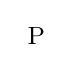
\begin{tikzpicture}
  \node[font=\small,inner sep=0pt] (n0) at (0,0) {P};
  \report{n0}{0}{{\small P}}
\end{tikzpicture}
\begin{tikzpicture}
  \node[font=\small,inner sep=0pt] (n1) at (0,0) {T};
  \report{n1}{1}{{\small T}}
\end{tikzpicture}
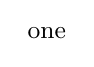
\begin{tikzpicture}
  \node[font=\small,inner sep=0pt] (n2) at (0,0) {one};
  \report{n2}{2}{{\small one}}
\end{tikzpicture}
\begin{tikzpicture}
  \node[font=\small,inner sep=0pt] (n3) at (0,0) {x};
  \report{n3}{3}{{\small x}}
\end{tikzpicture}
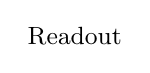
\begin{tikzpicture}
  \node[font=\small,inner sep=0pt] (n4) at (0,0) {Readout};
  \report{n4}{4}{{\small Readout}}
\end{tikzpicture}
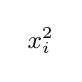
\begin{tikzpicture}
  \node[font=\small,inner sep=0pt] (n5) at (0,0) {$x_i^2$};
  \report{n5}{5}{{\small $x_i^2$}}
\end{tikzpicture}
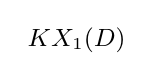
\begin{tikzpicture}
  \node[font=\small,inner sep=0pt] (n6) at (0,0) {$KX_1(D)$};
  \report{n6}{6}{{\small $KX_1(D)$}}
\end{tikzpicture}
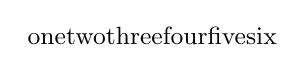
\begin{tikzpicture}
  \node[font=\small,inner sep=0pt] (n7) at (0,0) {one\\[3pt]two\\three\\four\\five\\six};
  \report{n7}{7}{{\small one\\[3pt]two\\three\\four\\five\\six}}
\end{tikzpicture}
\end{document}
